% !TEX root =  master.tex
\chapter{Vorbereitung der Daten}

Intel bietet auf ihrer Webseite die Möglichkeit unterschiedliche Prozessoren miteinander zu vergleichen.
Es werden alle Desktop-Prozessoren der Intel Core I7-Reihe an Prozessoren ausgewählt, damit es eine große Anzahl an Datensätzen gibt und auch die Spannweite zwischen gewissen Werten groß genug ist, dass Unterschiede leichter zu erkennen sind.
Z.B. ist die Kernanzahl pro Prozessor seit der 4. Generation stark gestiegen, wohingegen die Anzahl an Prozessorkernen bei Intel Core I3-Modellen nicht so stark angestiegen sind.
Die Daten werden direkt von \href{https://www.intel.de/content/www/de/de/products/compare.html?productIds=212279,212280,212047,212048,212251,199325,199335,199314,199316,199318,191048,191792,193738,190885,186604,148263,140642,126684,97129,93339,88200,88195,87718,88040,80807,80808,80809,80814,80806,77656,76642,75121,75122,75123,75124,75125,236781,236794,236854,236783,236789,230492,230490,230491,230500,230489,134596,134591,134592,134594,134595,129948,126686,97122,97128,88196}{Intels Webseite} bezogen.
Da Intel keine API anbietet, um deren CPU-Spezifikationen zu vergleichen und zu exportieren, muss die CSV-Datei selber heruntergeladen werden. 
Bevor die Daten aus der CSV ausgelesen werden können, müssen diese noch etwas aufbereitet werden.
Wie in Abbildung \ref{fig:intel_webseite} zu sehen ist, sind hier leider die Prozessormodelle die Spalten anstatt der Zeilen. 


Bevor die CSV bereinigen können, muss also die  Matrix der CSV noch einmal transponiert werden.
Sonst wären die einzelnen Prozessoren die Spalten in der Datenbank, wo die bereinigte Daten der CSV abgespeichert werden.
Weiterhin sind nicht alle Einträge in der CSV interessant für die Auswertung der Daten.
Viele der Einträge in der CSV listen nur Features oder Prozessorerweiterungen auf, die nicht einfach zu vergleichen sind oder sich nicht visualisieren lassen.
Weiterhin sind manche Einträge bei älteren Prozessoren komplett leer, weswegen die Datenmenge in diesen Spalten stark absinkt.
Daher werden nur ausgewählte Spalten ausgewählt, die interessant für die Fragestellung sind und auch genügend Datenpunkte haben.

\cleardoublepage

\begin{figure}
	\centering 
	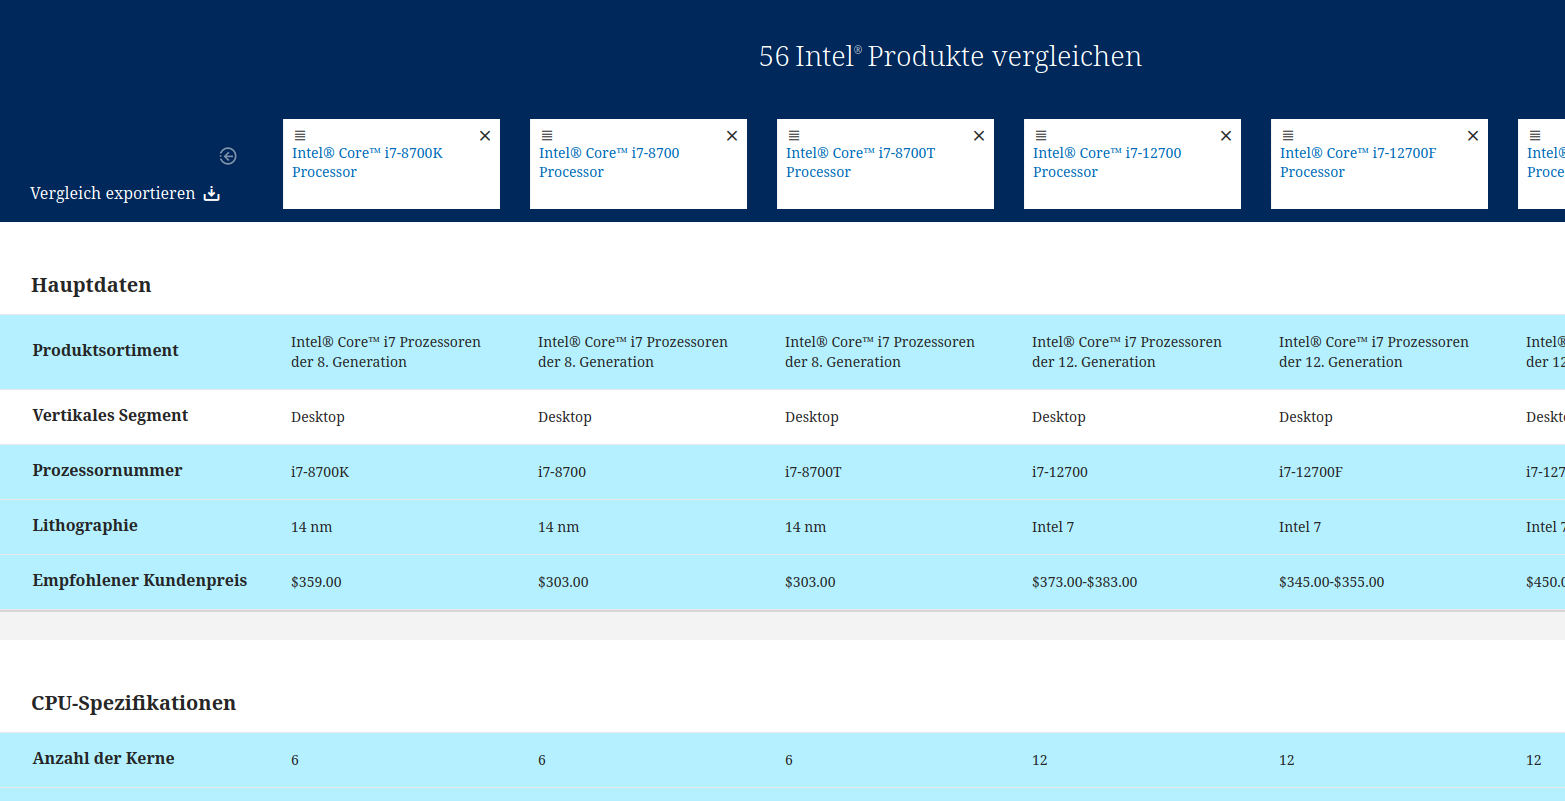
\includegraphics[width=\textwidth]{\imagedir/webseite.png} 
	\captionsetup{format=hang}
	\caption[Webseite von Intel]{\label{fig:intel_webseite}Webseite zum Produktvergleich von Intel-Prozessoren \\Quelle: \cite{i7_intel_2024}}
\end{figure}

Aufgrund der mächtigen Standardwerkzeugen eines POSIX-kompatiblen Betriebssystem wie Linux, wurde `awk` verwendet, um die Spalten in Zeilen umzubauen und umgekehrt.
`awk` arbeitet nicht nur mit Zeilen, wie z.B. `grep` oder `sed`, sondern kann auch in einzelnen Spalten filtern.
Normalerweise sind die Standardtrennzeichen von Spalten für `awk`  Leerzeichen und Tabulatoren. Es ist aber möglich mit dem `-F` Flag anzugeben, dass ein anderes Trennzeichen verwendet wird.
In `awk` wird normalerweise mit regulären Ausdrucken gefiltert, aber aufgrund einer statischen CSV-Datei kann direkt nach Spaltennamen sortiert werden.
Das entsprechende Skript sieht folgendermaßen aus:

\begin{lstlisting}[caption={\texttt{clean.sh}},captionpos=b]
#!/bin/bash

awk -F ',' '
NR==5   ||
NR==7   ||
NR==8   ||
NR==12  ||
NR==13  ||
NR==14  ||
NR==15  ||
NR==16  ||
NR==17  ||
NR==18  ||
NR==19  ||
NR==22  ||
NR==23  ||
NR==24  ||
NR==25  ||
NR==26  ||
NR==27  ||
NR==28  ||
NR==29  ||
NR==30  ||
NR==31  ||
NR==36  ||
NR==42  ||
NR==56  ||
NR==57  ||
NR==58  ||
NR==59  ||
NR==60  ||
NR==61  ||
NR==62  ||
NR==82  ||
NR==90 
{print $0}' "Intel_UPE_ComparisonChart_2024_11_04_i7.csv" |

awk '
{
	for (i=1; i<=NF; i++)  
	a[i] = a[i] ? a[i] "," $i : $i  
}
END {
	for (i=1; i in a; i++)  
	print a[i]
}
' FS=, OFS=, > clean.csv
\end{lstlisting}

Das Skript besteht aus zwei Teilen: Im ersten Teil werden die entsprechenden Spalten mit `awk` nach Spaltennummer ausgefiltert, welche vorher als interessant deklariert wurden, und in den zweiten Teil gepiped. 
Im zweiten Teil werden die jeweiligen Spalten in einer for-Schleife in neue Zeilen geladen. Nachdem die gesamte Datei eingelesen wurde, kann diese wieder transponiert ausgegeben werden. Nun kann mit dem eigentlichen Säubern der Daten begonnen werden.



